% Derived from the TeX Live PGF shapes.arrows manual's single/double-arrow examples.
\documentclass[border=2pt]{standalone}
\usepackage{tikz}
\usetikzlibrary{shapes.arrows,arrows.meta}
\begin{document}
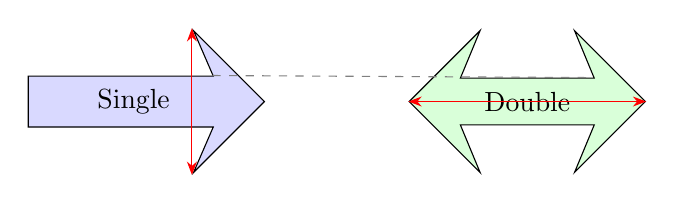
\begin{tikzpicture}[>=Stealth]
  \node[single arrow, draw, fill=blue!15,
    minimum height=3cm, minimum width=1.8cm,
    single arrow head extend=.5cm, single arrow head indent=.25cm] (single) at (0,0) {Single};
  \node[double arrow, draw, fill=green!15,
    minimum height=3cm, minimum width=1.8cm,
    double arrow head extend=.5cm, double arrow head indent=.25cm] (double) at (5,0) {Double};
  \draw[red, <->] (single.before tip) -- (single.after tip);
  \draw[red, <->] (double.tip 1) -- (double.tip 2);
  \draw[gray, dashed] (single.before head) -- (double.before head 1);
\end{tikzpicture}
\end{document}
